\subsection{Idea Space}

Identity, income, and asset verification is important for many banks and lenders. If verification is not done swiftly and correctly, then it can cost the lender. These costs can come in the form of being frauded out of money, losing loan applicants to competitors due to slow processing times, and additional time processing for their verifications team. As of 2020, most lenders still have their verification done by teams of human verifiers. Humans being prone to inane mistakes and operating thousands of times slower than a computer is another issue that probed the idea of a verifications system.

\subsection{Similar Ideas}

\begin{wrapfigure}{R}{0.5\textwidth}
    \centering
    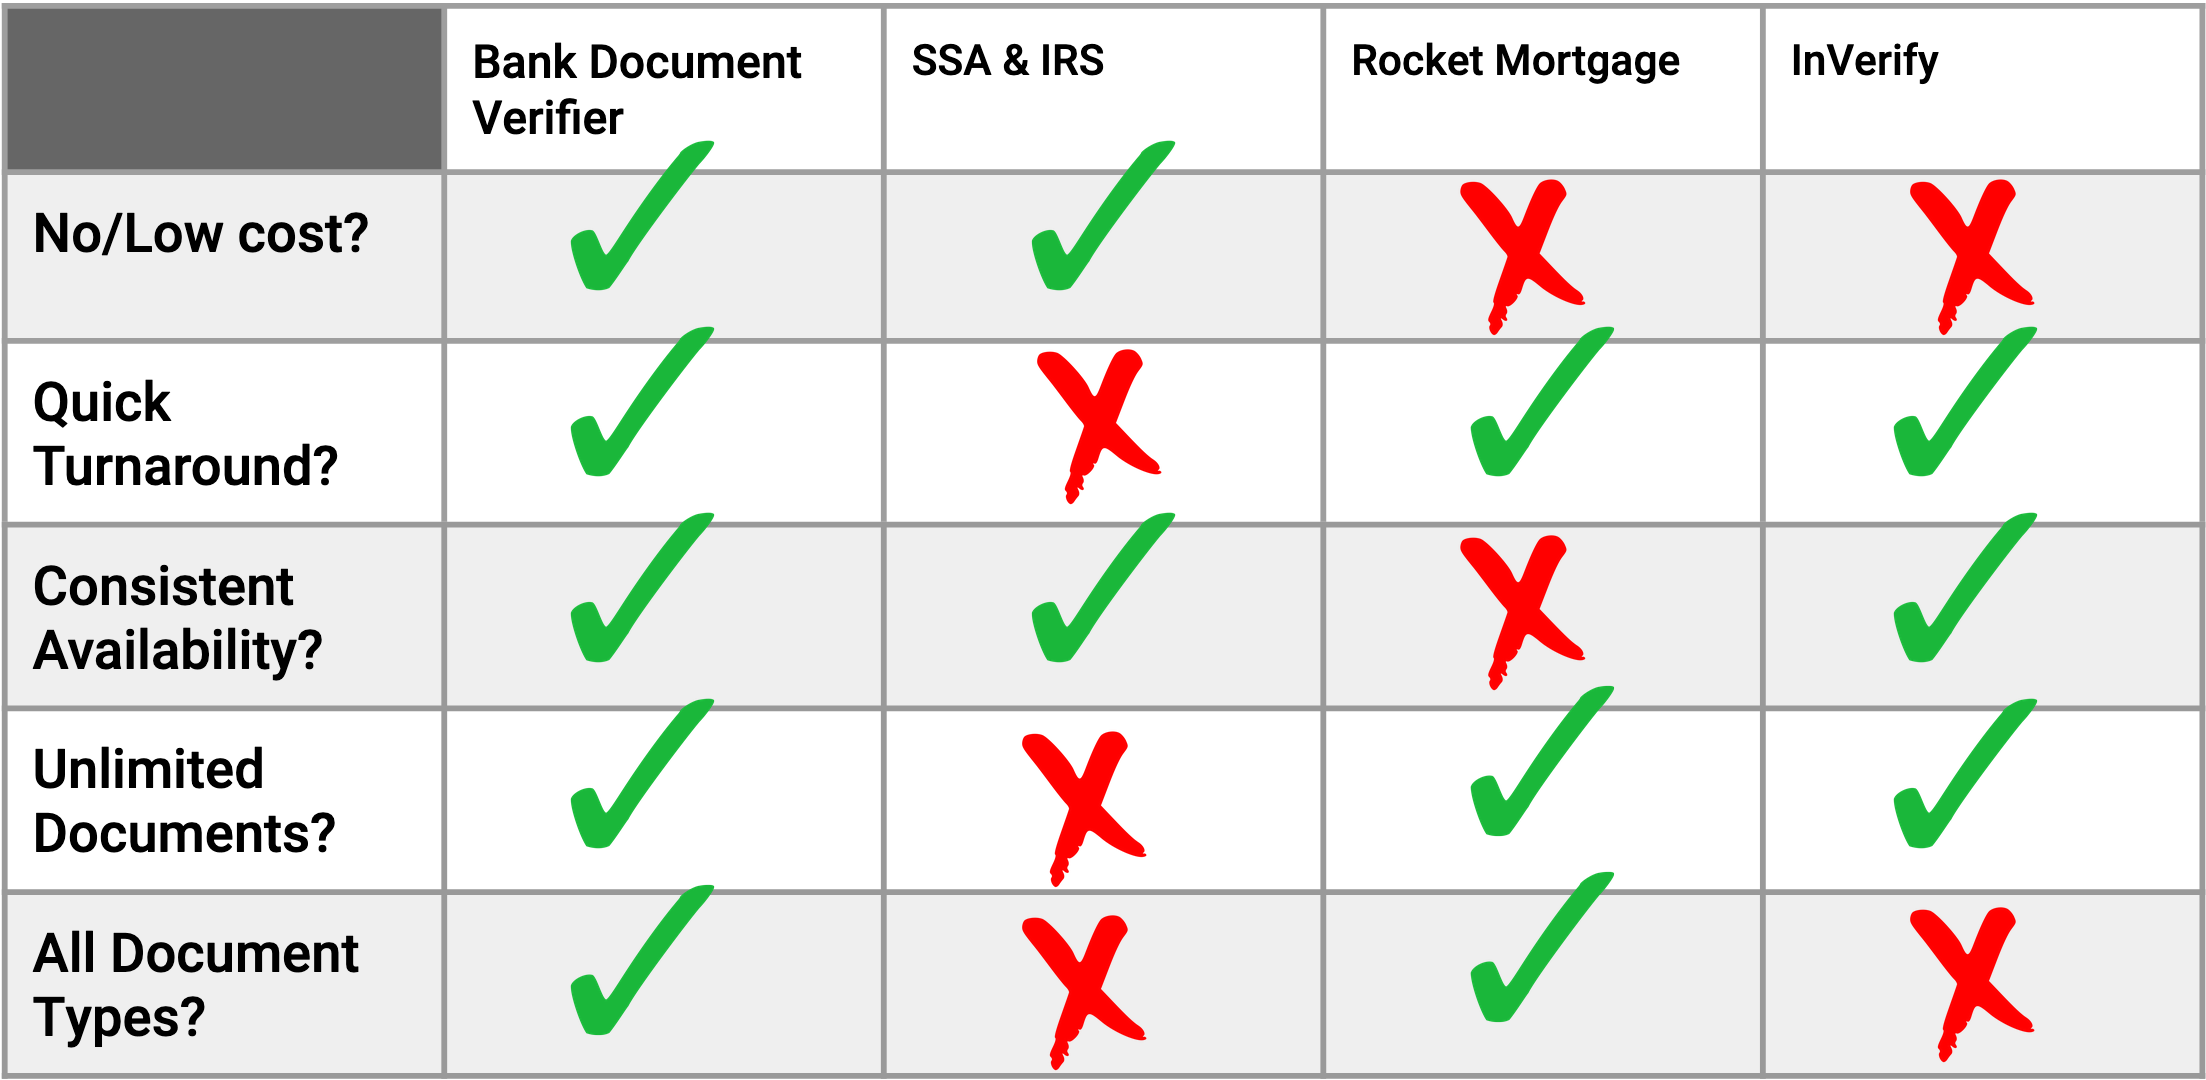
\includegraphics[width=0.48\textwidth]{assets/comparison-table.png}
    \caption{How our system compares with others}
\end{wrapfigure}

Since this problem has existed in the financial industry for a long time, there do exist verification systems out there. But most of them have issues with either speed, consistency, or generality. Our customer base is going to need a plethora of documents to be verified and, as such, we want to be able to scan all of them efficiently. Many of the current products will scan fast and accurately, but those tend to not scan all document types. The SSA and IRS also offer options, but they limit how many documents can be verified at once and are extremely slow. We believe the Bank Document Verifier will be able to cover what these other companies have lacked.

\subsection{Required Technology}

In order to create a modern, flexible, tried-and-tested, and secure web application, it is essential that we thoughtfully consider frameworks and platforms that fit this requirement. After extensive research, we determined that NEXT.js would be an excellent option as a development framework for our front-end. Some advantages of NEXT.js include: 

\begin{itemize}
    \item Optimal performance/stability
    \item A modular architecture, allowing for free and interchangeable functions which we can reuse across the code base
    \item A large community of support, showing that the framework is clearly tried-and-tested
    \item The ability to integrate easily with Node.js for our backend
\end{itemize}

The back-end will be written in both Node.js and Python, where we will be using Python to handle document parsing and text extraction, and Node.js to handle strict server I/O operations. Each platform suits its respective task well, so we are confident in our decision here.

Files will be stored locally in the directory for interrim data files that are part of a pipeline. Any data that needs persistence will be stored in our Mongo Database. Persistent data will include Documents and Login information.

\subsection{Assets}

There is an API called Accurint that can be used to verify many forms of identification. Many of the projects we saw in our research used that to a high degree of success but stopped short of having all the features we’d like. We will not be using Accurint directly but through the Bank's API. Achieving the Core functionality without accessing the API in our code and instead, we will access the Bank's API.

While the demoable version of the Bank Document Verifier will feature the ability to create accounts using \href{https://next-auth.js.org/}{Next-Auth}, the production version will simply hook into financial institution systems for accounts. This means that clients (who work for their respective financial institutions) will not be able to create their own accounts, and should reach out to their workplace's IT department for account creation. This emphasizes leaving accounts in control of the financial institution to minimize difficulties with migration.

\subsection{Hardware/Software Requirements}

Due to our program’s ease of incorporation into current financial institutions, as well as its relative programmatic simplicity, we will not require any hardware or software beyond what the institution already has in each of its computers (Windows 10, a mid-range processor, and, comfortably, 4 GB+ of RAM as well as 5 GB+ of storage).   